\subsection{Development evidence for checkpoint assessment}

The development cohorts explain why candidate-cost differences were not used as substitutes for deployment outcomes. In A, extending a direct scorer from 250 to 1,000 total steps reduced its mean FV candidate-cost difference from $5.6138\times10^{-7}$ to $1.4751\times10^{-7}$, while mean closed-loop cost increased from 0.0299374 to 0.0480506 on the same eight validation episodes. Five of six nominal episodes worsened; two initially hot episodes tied. Both comparisons had no deadline misses. The learning-rate schedule also changed, so this is a checkpoint comparison rather than an isolated training-duration effect.

In B, minimum candidate-cost difference and rollout-based validation criteria selected different checkpoints in all five scorer families. Selected nominal validation costs were 5.09--68.17\% lower despite larger candidate-cost differences. These estimates reuse selection episodes and cannot establish independent selector benefit. A sensor-only checkpoint selected by the offline criterion produced new limit violations in 11 of 40 validation trajectories spanning three episodes. Only the rollout-selected policies received the separate test evaluation; their results do not supply the missing comparison against unselected alternatives. The supplementary record retains the selection rules, candidate histories, and protocol identifiers.

These observations motivate checking the downstream criterion. They do not validate a general checkpoint selector or explain D's residual comparison. The short held-action FV cost also uses eligibility rules that differ from the calibrated deployed gate; its small numerical difference is not a bound on 60-second feedback error or a solver-accuracy estimate.

\subsection{A selected command-divergence diagnostic}

Cohort C uses a frozen direct scorer and one post hoc selected episode, separately from D. At the original 10-ms plant cap, normal-path delays of 13, 38, and 50~ms yield costs of 0.0362894, 0.0099116, and 0.0366019 without deadline misses. The 38-ms case was selected because it accounts for 100.71\% of the net replay degradation across nine fresh nominal confirmation episodes; it is not a representative population estimate. At the first differing requests (1.4 and 2.7~s), eligibility masks match and the gate does not intervene. Individual heater commands differ before their request-aligned mean does. Supplement S1 retains those command vectors, timing plots, and score margins.

Recomputed closed-loop decisions remain sensitive to the plant step. The lowest-cost delay changes from 38 to 50 to 13~ms as the cap decreases from 10 to 5 to 2.5~ms (Fig.~\ref{fig:numericalC}). All nine runs complete without deadline misses. In contrast, holding each original applied-command sequence fixed gives cost changes below 0.0032\% from 10 to 1.25~ms. Across 1-Hz full-field samples, the largest RMSE is $6.25\times10^{-4}$~K and the largest pointwise difference is $3.62\times10^{-3}$~K. Successive refinement differences approximately halve; they are not bounds on the continuous-time solution.

\begin{figure}[tbp]
\centering
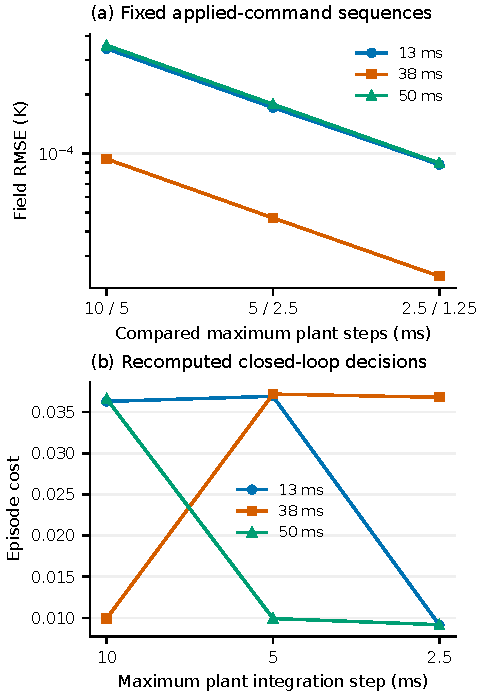
\includegraphics[width=\linewidth]{figures/numerical_case_C.pdf}
\caption{Numerical sensitivity of the selected C episode. (a) Temperature-field RMSE between successive plant-step refinements, sampled at 1~Hz with original applied commands fixed. (b) Costs with closed-loop decisions recomputed at each cap. Colors identify normal-path delay conditions.}
\label{fig:numericalC}
\end{figure}

Small fixed-input differences coexist with much larger feedback changes. This is consistent with amplification through discrete action selection, but does not establish a unique numerical mechanism or an optimal physical delay. C is a supporting sensitivity diagnostic; the D comparisons concern different frozen residual systems.

